\documentclass[12pt]{article}
\usepackage[left=.5in, right=.5in, top=.5in, bottom=.5in]{geometry}
\usepackage[parfill]{parskip}
\usepackage{amsmath, amssymb, graphicx, svg}
\pagenumbering{gobble}
\setlength\parindent{0pt}
\newcommand{\E}{\mathbb{E}}
\newcommand{\m}[1]{\mathbf{#1}}
\newcommand{\mhat}[1]{\hat{\mathbf{#1}}}
\newcommand{\mep}{\boldsymbol{\epsilon}}
\newcommand{\ol}[1]{\overline{#1}}
\newcommand{\tr}{\text{tr}}

\begin{document}

\begin{center}
{\Large CSC413H1 - Assignment 1}
\end{center}

\textbf{1.2.1:} Training converges when $\frac{1}{n}||X\mhat w-\m t||^2_2$ achieves its minimum, or equivalently when $\nabla_{\mhat w} \frac{1}{n}||X\mhat w-\m t||^2_2 = \frac{2}{n}X^T(X\mhat w -\m t) = 0$. To solve for $\mhat w$ in this scenario, note that
\begin{align*}
    \frac{2}{n}X^T(X\mhat w -\m t) = 0 \iff X^T(X\mhat w -\m t) = 0 \iff X^T X\mhat w = X^T \m t.
\end{align*}
Since $d < n, X^T X$ is invertible, we can multiply $(X^T X)^{-1}$ to both sides to yield
\begin{align*}
    (X^T X)^{-1} X^T X\mhat w = \mhat w = (X^T X)^{-1} X^T \m t.
\end{align*}

\textbf{1.2.2:} Substituting the previous answer and $\m t = X\m w^* + \mep$ into the loss yields
\begin{align*}
    \frac{1}{n}||X\mhat w - \m t||^2_2 &= \frac{1}{n}||X(X^T X)^{-1}X^T\m t - \m t||^2_2 = \frac{1}{n}||X(X^T X)^{-1}X^T (X\mhat w + \mep) - (X\mhat w + \mep)||^2_2\\
    &= \frac{1}{n}||X(X^T X)^{-1}X^T X\mhat w + X(X^T X)^{-1}X^T\mep - X\mhat w - \mep||^2_2\\
    &= \frac{1}{n}||X\mhat w - X\mhat w + (X(X^T X)^{-1}X^T - I)\mep||^2_2\\
    &= \frac{1}{n}||(X(X^T X)^{-1}X^T - I)\mep||^2_2
\end{align*} as desired. Notice that this equals
\begin{multline*}
    \frac{1}{n}(X(X^T X)^{-1}X^T\mep - \mep)^T(X(X^T X)^{-1}X^T\mep - \mep) \\ = \frac{1}{n}(\mep^T X(X^T X)^{-1}X^T\mep - \mep^T X(X^T X)^{-1}X^T\mep - \mep^T X(X^T X)^{-1}X^T\mep + \mep^T\mep) = \mep^T\mep - \mep^T X(X^T X)^{-1}X^T\mep
\end{multline*} since $((X^T X)^{-1})^T = ((X^T X)^T)^{-1} = (X^T X)^{-1}$. Then, the expectation of this error is
\begin{align*}
    \frac{1}{n}\E\Big[\mep^T\mep - \mep^T X(X^T X)^{-1}X^T\mep\Big] &= \frac{1}{n}\E\Big[\tr(\mep\mep^T - \mep^T X(X^T X)^{-1}X^T\mep)\Big] \text{ since the inside is a scalar}\\
    &= \frac{1}{n}\E\Big[\tr(\mep^T\mep)\Big] - \frac{1}{n}\E\Big[\tr(\mep^T X(X^T X)^{-1}X^T\mep\Big] \text{ by linearity of trace}\\
    &= \frac{1}{n}\tr\Big[\E(\mep^T\mep)\Big] - \frac{1}{n}\tr\Big[\E(\mep^T X(X^T X)^{-1}X^T\mep)\Big] \text{ since }\E[\tr(A)] = \tr[\E(A)]\\
    &= \frac{1}{n}\tr\Big[\E(\Sigma_{i=1}^n \mep^2_i)\Big] - \frac{1}{n}\tr\Big[\E(\mep\mep^T X(X^T X)^{-1}X^T)\Big]\\
    &= \frac{1}{n}\tr\Big[\Sigma_{i=1}^n\E(\mep^2_i)\Big] - \frac{1}{n}\tr\Big[\E(\mep\mep^T) X(X^T X)^{-1}X^T\Big] \text{ by independence}\\
    &= \frac{1}{n}\tr(n\sigma^2) - \frac{1}{n}\tr\Big[\sigma^2 X(X^T X)^{-1}X^T\Big]\\
    &= \sigma^2 - \frac{\sigma^2}{n}\tr\Big[(X^T X)^{-1}X^T X\Big]\\
    &= \sigma^2 - \frac{\sigma^2 d}{n}
\end{align*} where $\E(\mep^2_i) = \text{Var}(\mep_i) + \E(\mep_i)^2 = \sigma^2$ and $\E(\mep\mep^T) = \begin{bmatrix} \E(\mep^2_1) & \dots & \E(\mep_1)\E(\mep_n) \\ \vdots & \ddots & \vdots \\ \E(\mep_n)\E(\mep_1) & \dots & \E(\mep^2_n) \end{bmatrix} = \sigma^2 I_n$.

\textbf{1.3.1:} $\mhat{w}^T\m{x_1} = \begin{bmatrix}\hat{w_1} & \hat{w_2}\end{bmatrix}\begin{bmatrix}1 \\ 1\end{bmatrix} = \hat{w_1} + \hat{w_2} = t_1 = 3$, so the equation of the line is $\hat{w_2} = -\hat{w_1} + 3$. Thus, there are infinitely many $\mhat{w}$ satisfying $\mhat{w}^T\m{x_1} = t_1$.

\textbf{1.3.2:} Assuming that the gradient is spanned by the rows of $X$, we substitute $\mhat w = X^T\m{a}$ for $\m a \in \mathbb{R}^n$ into the objective from 1.2.1 to yield
\begin{align*}
     X^T(X\mhat w - \m t) = 0 &\iff (XX^T)^{-1}XX^T(X\mhat w - \m t) = 0 \iff X\mhat w -\m t = 0 \iff XX^T\m a -\m t = 0\\
     &\iff XX^T\m a = \m t \iff \m a = (XX^T)^{-1}\m t
\end{align*} where the first and last equivalences hold since $d > n$ and $XX^T$ is invertible. Thus, the unique minimizer is
\begin{align*}
    \mhat w = X^T\m a = X^T(XX^T)^{-1}\m t.
\end{align*}

\textbf{1.3.4:} The plot of the polynomials and the plot of the test losses vs. degree of polynomial are as follows:
\begin{center}
    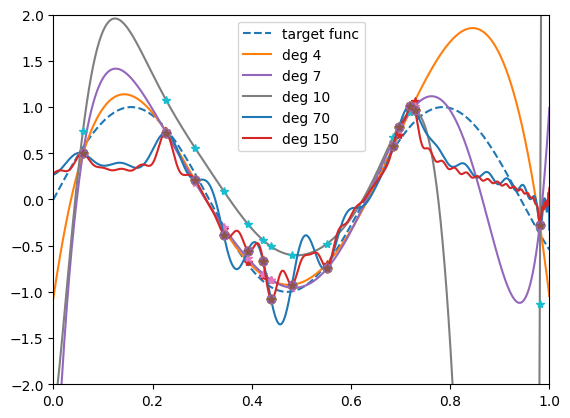
\includegraphics[scale=.75]{1.3.4-1.png}
    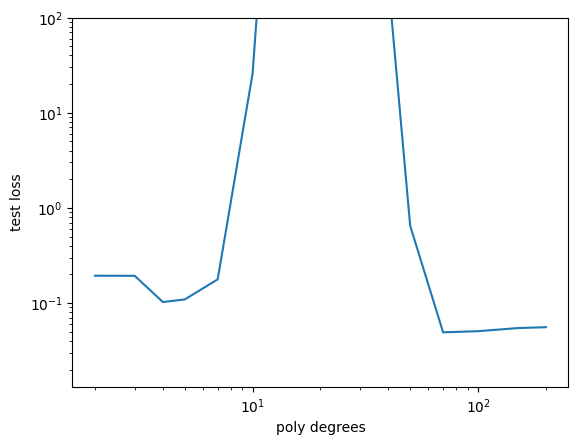
\includegraphics[scale=.75]{1.3.4-2.png}
\end{center}

Overparameterization does not always lead to overfitting. As shown in the last plot, the test loss decreases when the degree of polynomial is around $10^2$, indicating that a higher degree polynomial does not always have a higher test error.

\textbf{2.1.2:} Suppose that $\m x$ has dimensions $D \times 1$ and $\m z_1, \m h_1, \m z_2, \m h_2, \m g$ have dimensions $K \times 1$. Define $\m h_{1i}$ as the $i$-th component of $\m h_1$ and similarly for $\m z_{1i}, \m h_{2i}, \m z_{2i}$.
\begin{align*}
    \ol{\mathcal{J}} &= 1\\
    \ol{\mathcal{S}} &= -\ol{\mathcal{J}}\\
    \ol{\m y}' &= \begin{bmatrix} \dfrac{\partial S}{\partial\m y'_1} & \dots & \dfrac{\partial S}{\partial\m y'_N} \end{bmatrix}^T \ol{\mathcal{S}} = \begin{bmatrix} 0 & \dots & \dfrac{1}{\m y_t'} & \dots & 0 \end{bmatrix}^T \ol{\mathcal{S}}\\
    \ol{\m y} &= \begin{bmatrix} \dfrac{\partial\m y'_1}{\partial\m y_1} & \dots & \dfrac{\partial\m y'_1}{\partial\m y_N} \\ \vdots & \ddots & \vdots \\ \dfrac{\partial\m y'_N}{\partial\m y_1} & \dots & \dfrac{\partial\m y'_N}{\partial\m y_N} \end{bmatrix}^T \ol{\m y}' = \text{softmax}'(\m y)^T \ol{\m y}'\\
    \ol{\m g} &= \begin{bmatrix} \dfrac{\partial\m y_1}{\partial\m g_1} & \dots & \dfrac{\partial\m y_1}{\partial\m g_K} \\ \vdots & \ddots & \vdots \\ \dfrac{\partial\m y_N}{\partial\m g_1} & \dots & \dfrac{\partial\m y_N}{\partial\m g_K} \end{bmatrix}^T \ol{\m y} = \m W^{(3)T} \ol{\m y}\\
    \ol{\m h_1} &= \begin{bmatrix} \m h_{21}\ol{\m g_1} \\ \vdots \\ \m h_{2K}\ol{\m g_K} \end{bmatrix} = \m h_2 \circ \ol{\m g}\\
    \ol{\m h_2} &= \begin{bmatrix} \m h_{11}\ol{\m g_1} \\ \vdots \\ \m h_{1K}\ol{\m g_K} \end{bmatrix} = \m h_1 \circ \ol{\m g}\\
    \ol{\m z_1} &= \begin{bmatrix} \mathbb{I}(\m z_{11} > 0) \\ \vdots \\ \mathbb{I}(\m z_{1K} > 0) \end{bmatrix} \circ \ol{\m h_1} \text{ where }\mathbb{I}\text{ is the indicator function}\\
    \ol{\m z_2} &= \begin{bmatrix} \sigma(\m z_{21}) \\ \vdots \\ \sigma(\m z_{2K}) \end{bmatrix} \circ \begin{bmatrix} 1 - \sigma(\m z_{21}) \\ \vdots \\ 1 - \sigma(\m z_{2K}) \end{bmatrix} \circ \ol{\m h_2}\\
    \ol{\m x} &= \begin{bmatrix} \dfrac{\partial\m y_1}{\partial\m x_1} & \dots & \dfrac{\partial\m y_1}{\partial\m x_D} \\ \vdots & \ddots & \vdots \\ \dfrac{\partial\m y_N}{\partial\m x_1} & \dots & \dfrac{\partial\m y_N}{\partial\m x_D} \end{bmatrix}^T \ol{\m y} + \begin{bmatrix} \dfrac{\partial\m z_{11}}{\partial\m x_1} & \dots & \dfrac{\partial\m z_{11}}{\partial\m x_D} \\ \vdots & \ddots & \vdots \\ \dfrac{\partial\m z_{1K}}{\partial\m x_1} & \dots & \dfrac{\partial\m z_{1K}}{\partial\m x_D} \end{bmatrix}^T \ol{\m z_1} + \begin{bmatrix} \dfrac{\partial\m z_{21}}{\partial\m x_1} & \dots & \dfrac{\partial\m z_{21}}{\partial\m x_D} \\ \vdots & \ddots & \vdots \\ \dfrac{\partial\m z_{2K}}{\partial\m x_1} & \dots & \dfrac{\partial\m z_{2K}}{\partial\m x_D} \end{bmatrix}^T \ol{\m z_2} \\
    &= \m W^{(4)T} \ol{\m y} + \m W^{(1)T} \ol{\m z_1} + \m W^{(2)T} \ol{\m z_2}
\end{align*}

\textbf{2.2.1:}
\begin{align*}
    \m z &= \begin{bmatrix} 1 & 2 & 1 \\ -2 & 1 & 0 \\ 1 & -2 & -1 \end{bmatrix} \begin{bmatrix} 1 \\ 3 \\ 1 \end{bmatrix} = \begin{bmatrix} 8 \\ 1 \\ -6 \end{bmatrix}\\
    \m h &= \text{ReLU}(\m z) = \begin{bmatrix} 8 \\ 1 \\ 0 \end{bmatrix}\\
    \ol{\m h} &= \begin{bmatrix} \dfrac{\partial\m y_1}{\partial\m h_1} & \dots & \dfrac{\partial\m y_1}{\partial\m h_3} \\ \vdots & \ddots & \vdots \\ \dfrac{\partial\m y_3}{\partial\m h_1} & \dots & \dfrac{\partial\m y_3}{\partial\m h_3} \end{bmatrix} \ol{\m y} = \m W^{(2)T} \ol{\m y} = \begin{bmatrix} -2 & 1 & -3 \\ 4 & -2 & 4 \\ 1 & -3 & 6 \end{bmatrix}\begin{bmatrix} 1 \\ 1 \\ 1 \end{bmatrix} = \begin{bmatrix} -4 \\ 6 \\ 4 \end{bmatrix}\\
    \ol{\m z} &= \begin{bmatrix} \mathbb{I}(\m z_1 > 0) \\ \mathbb{I}(\m z_2 > 0) \\ \mathbb{I}(\m z_3 > 0) \end{bmatrix} \circ \ol{\m h} = \begin{bmatrix} 1 \\ 1 \\ 0 \end{bmatrix} \circ \begin{bmatrix} -4 \\ 6 \\ 4 \end{bmatrix} = \begin{bmatrix} -4 \\ 6 \\ 0 \end{bmatrix}\\
    \ol{\m W^{(1)}} &= (\ol{\m z} \m x^T)^T = (\begin{bmatrix} -4 \\ 6 \\ 0 \end{bmatrix} \begin{bmatrix} 1 & 3 & 1 \end{bmatrix})^T = \begin{bmatrix} -4 & 6 & 0 \\ -12 & 18 & 0 \\ -4 & 6 & 0 \end{bmatrix}\\
    \ol{\m W^{(2)}} &= (\ol{\m y} \m h^T)^T = (\begin{bmatrix} 1 \\ 1 \\ 1 \end{bmatrix} \begin{bmatrix} 8 & 1 & 0 \end{bmatrix})^T = \begin{bmatrix} 8 & 8 & 8 \\ 1 & 1 & 1 \\ 0 & 0 & 0 \end{bmatrix}\\
    ||\ol{\m W^{(1)}}||^2_F &= \text{trace}(\begin{bmatrix} -4 & -12 & -4 \\ 6 & 18 & 6 \\ 0 & 0 & 0 \end{bmatrix} \begin{bmatrix} -4 & 6 & 0 \\ -12 & 18 & 0 \\ -4 & 6 & 0 \end{bmatrix}) = 572\\
    ||\ol{\m W^{(2)}}||^2_F &= \text{trace}(\begin{bmatrix} 8 & 1 & 0 \\ 8 & 1 & 0 \\ 8 & 1 & 0 \end{bmatrix} \begin{bmatrix} 8 & 8 & 8 \\ 1 & 1 & 1 \\ 0 & 0 & 0 \end{bmatrix}) = 195
\end{align*}

\textbf{2.2.2:}
\begin{align*}
    ||\ol{\m W^{(1)}}||^2_F &= ||\m x||^2_2 ||\ol{\m z}||^2_2 = (1^2 + 3^2 + 1^2)((-4)^2 + 6^2) = (11)(52) = 572\\
    ||\ol{\m W^{(2)}}||^2_F &= ||\m h||^2_2 ||\ol{\m y}||^2_2 = (8^2 + 1^2)(1^2 + 1^2 + 1^2) = (37)(3) = 195
\end{align*}

\textbf{2.2.3:}
\begin{tabular}{|c|c|c|c|c|} 
    \hline
    & T (Naive) & T (Efficient) & M (Naive) & M (Efficient) \\ 
    \hline
    Forward pass & $NKD^2$ & $NKD^2$ & $O(KD^2 + NKD)$ & $O(KD^2 + NKD)$ \\
    \hline
    Backward pass & $2NKD^2$ & $NKD^2$ & $O(NKD^2)$ & $O(KD^2 + NKD)$ \\
    \hline
    Gradient norm & $NKD^2$ & $NK(2D + 1)$ & $O(NKD^2)$ & $O(NKD)$\\
    \hline
\end{tabular}
\begin{itemize}
    \item Forward pass:
    \begin{itemize}
        \item For both the naive and efficient methods, there are $D^2$ scalar multiplications per weight matrix and input vector, and there are $K$ matrices and $N$ vectors, resulting in $NKD^2$ overall.
        \item Both methods need to store these $K$ matrices with $D^2$ parameters each ($O(KD^2)$) and $NK$ vectors with $D$ parameters each ($O(NKD)$).
    \end{itemize}
    \item Backward pass:
    \begin{itemize}
        \item Similar to the forward pass, both methods require $D^2$ scalar multiplications for each of $K$ matrices and $N$ vectors to calculate the error vectors. However, the naive method also needs to compute $NK$ Jacobians of the weights, each of which is an outer product with $D^2$ scalar multiplications.
        \item The naive method needs to store the activations ($O(NKD)$), error vectors ($O(NKD)$), weights ($O(KD^2)$), and the Jacobians of the weights ($O(NKD^2)$), resulting in $O(NKD^2 + KD^2 + 2NKD)$ or $O(NKD^2)$ overall. However, the efficient method does not need to store the Jacobians, resulting in $O(KD^2 + 2NKD)$ or $O(KD^2 + NKD)$ overall.
    \end{itemize}
    \item Gradient norm:
    \begin{itemize}
        \item The naive method requires $D^2$ scalar multiplications to calculate the norm for each of $NK$ Jacobians, while the efficient method only requires $2D$ multiplications to calculate the norm, plus an additional multiplication at the end, for each of $NK$ Jacobians.
        \item The naive method needs to store $NK$ Jacobians with $D^2$ parameters each ($O(NKD^2)$), while the efficient methods only needs to store $NK$ vectors with $D$ parameters each ($O(NKD)$).
    \end{itemize}
\end{itemize}

\textbf{3.1:} $\m{W}^{(1)} = \begin{bmatrix} 1 & 1 \\ 1 & -1 \end{bmatrix}$, $\m{W}^{(2)} = \begin{bmatrix} \frac{1}{2} & -\frac{1}{2} \\ \frac{1}{2} & \frac{1}{2} \end{bmatrix}$, $\m{b}^{(1)} = \m{b}^{(2)} = \begin{bmatrix} 0 \\ 0 \end{bmatrix}$, $\varphi^{(1)}(z) = |z|$, $\varphi^{(2)}(z) = z$.

\textbf{3.2:} Using merge sort: \begin{center}\includesvg[scale=.75]{3.2.svg}\end{center}

\end{document}
